\section{A Semantic Wiki for Science}

\begin{wrapfigure}{r}{4.2cm}
  \centering
  \vspace{-.9cm}
  \begin{tikzpicture}
    \node (s) at (0,0) {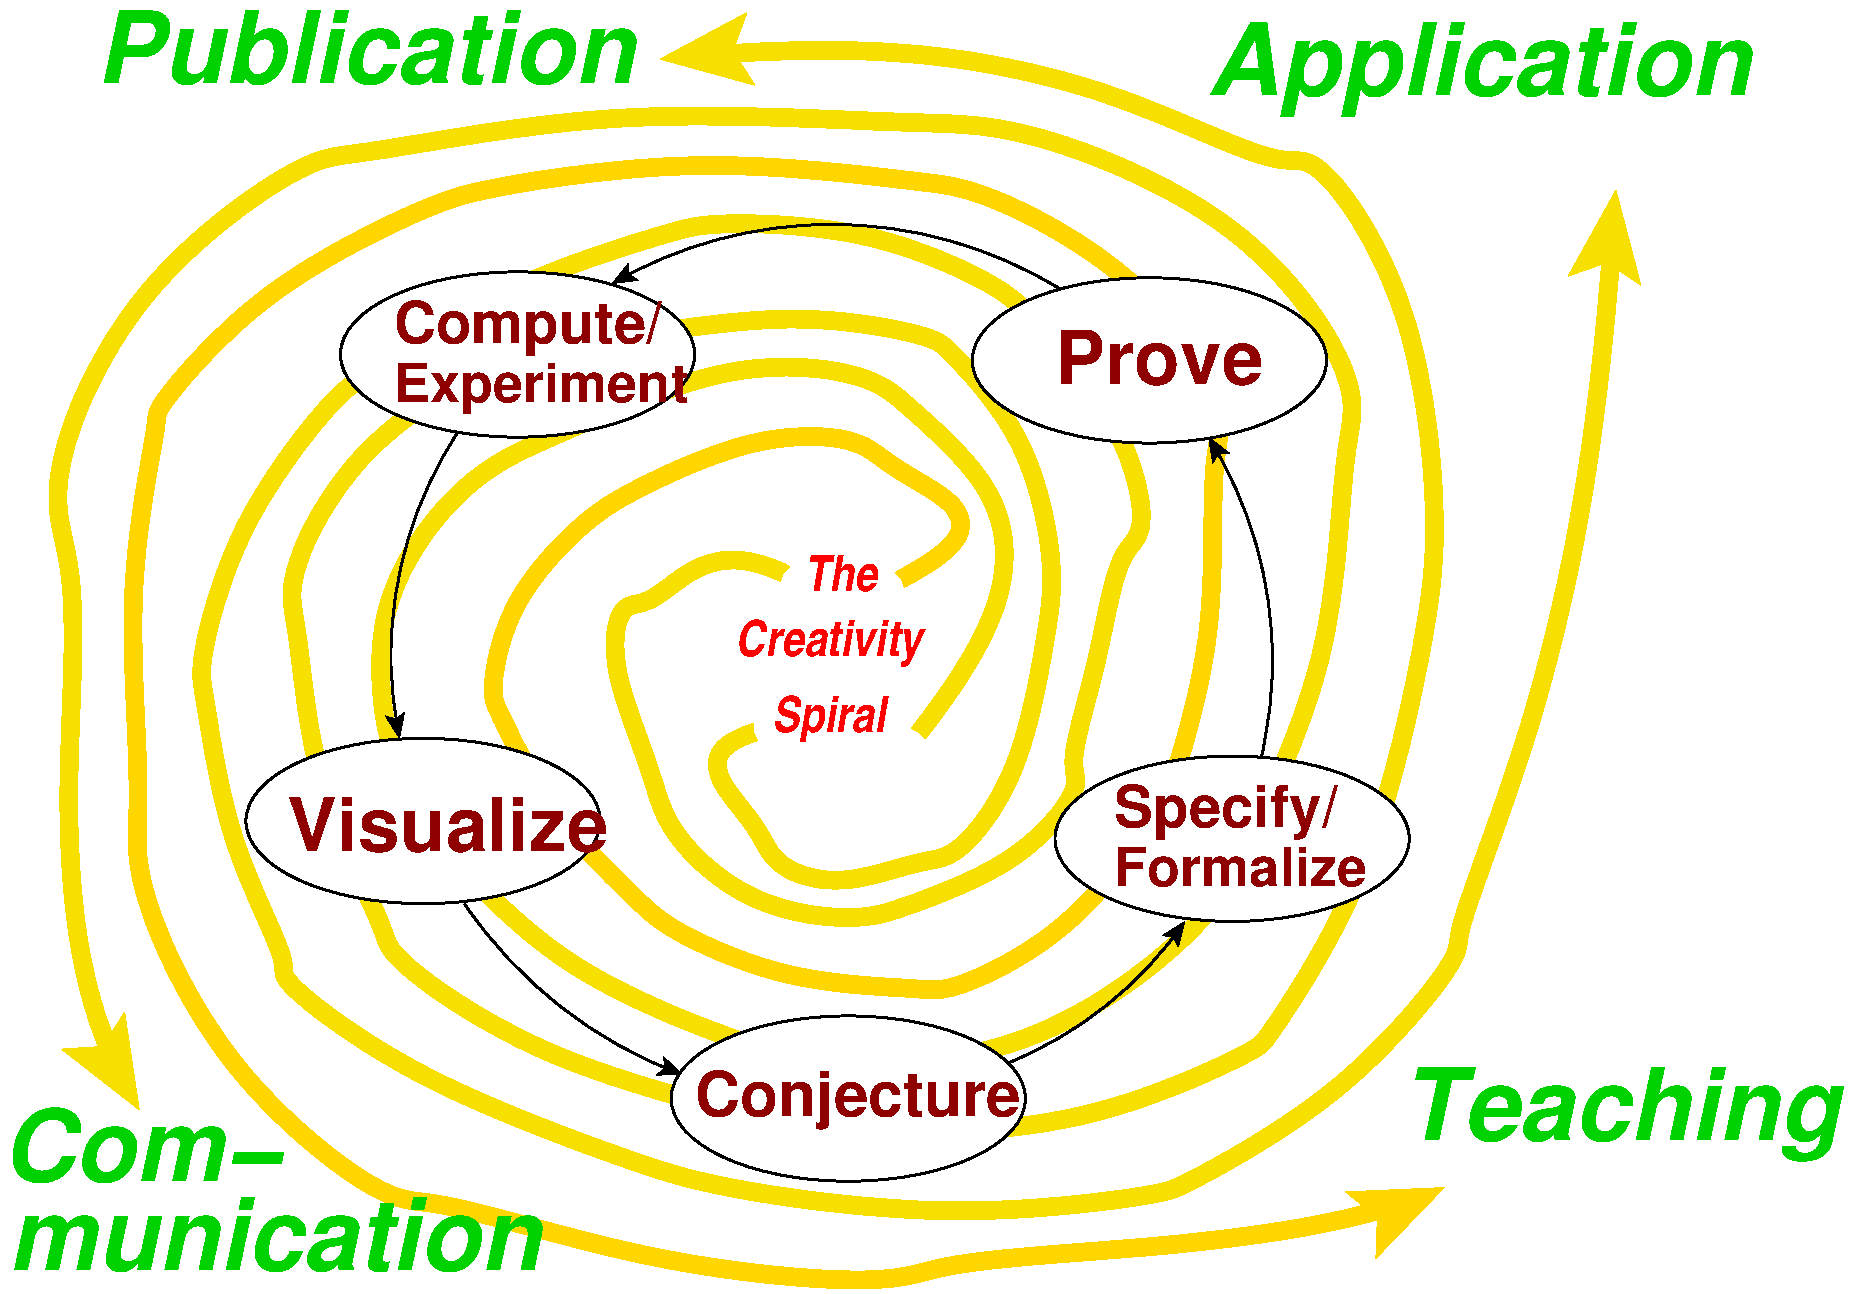
\includegraphics[width=4cm]{creativity-spiral}};
    \node at (s.south) {\scriptsize (B.\ Buchberger 1995)};
  \end{tikzpicture}
  \vspace{-1.2cm}
\end{wrapfigure}
Documents are the most important medium in science, if we assume a broad definition of
``document'', including any materialized item of (scientific) knowledge.  Scientific
communication mainly consists of exchanging documents---from informal drafts circulating
inside a working group to published, well-structured books.  A great deal of scientific
work consists of collaboratively authoring these documents---taking down first hypotheses,
commenting on results of experiments or project steps, as well as structuring, annotating,
and re-organizing existing items of knowledge.  Tools that
\emph{understand} the knowledge contained in scientific documents are desirable for
editing such documents.  One approach towards this is writing scientific documents in a
semantic markup language with an editor that knows the structures available in this
language.

Besides generic approaches like SALT~\cite{Groza:SALT07}, semantic markup has been most
deeply investigated in the specific domain of mathematics with ``long tradition in the
pursuit of conceptual clarity and representational rigor''~\cite{Kohlhase:omdoc1.2},
resulting in languages like MathML~\cite{CarlisleEd:MathML07},
OpenMath~\cite{BusCapCar:2oms04}, and OMDoc~\cite{Kohlhase:omdoc1.2}.  OMDoc is a language
that employs Content MathML
\ednote{I don't think we want this footnote.  It uses space, and if the users
  are curious about the difference, which doesn't seem relevant to our papre, they
  can look it up.}
\footnote{MathML comes in two flavors: Presentation MathML
  expresses the way a formula is rendered, whereas Content MathML models its logical
  structure.  Formal mathematical software like a Computer Algebra System would export
  formulae in Content MathML, but for publishing, they would be converted to Presentation
  MathML.} 
or OpenMath for structurally representing mathematical \emph{objects} (symbols,
numbers, equations, etc.) and adds two layers on top of that: Objects or informal text can
be annotated as mathematical \emph{statements} (symbol declarations, definitions, axioms,
theorems, proofs, examples, etc.), and collections of interrelated statements are grouped
into \emph{theories}.

With SWiM, a semantic wiki for mathematical knowledge management (see
section~\ref{sec:swim}), we have investigated collaborative editing of OMDoc documents.
It has turned out that a wiki is a suitable tool for supporting the workflow of
incremental formalization inherent to scientific writing.  But wikis have not only shown
to be appropriate for \emph{writing}, but also for project management, e.\,g.\ in
corporate settings~\cite{leuf01:wikiway}.  Thus, we are interested in applying our
technologies to scientific knowledge engineering projects.  

The Flyspeck project
introduced in section~\ref{sec:flyspeck} is particularly appealing as a use case
for a number of reasons. It
involves both highly formal and semi-formal mathematical knowledge.   
The proof contains descriptive and motivating yet informal text that would
be difficult to present in a strictly formal setting.
Finally, its purpose is to develop a scientific document---a formal proof of the Kepler
conjecture--- and to communicate this proof to the public.  Its large extent and the
required manpower suggest ``crowdsourcing'' the workload and supporting the project
organization by social software.  For example, doing this publicly on the web will contribute to
communicating the parts of the proof already done.  We are going to investigate whether
the three conditions for successful peer production stated by Tapscott and
Williams~\cite{wikinomics} will hold or can be satisfied by software support.
The conditions are
\begin{enumerate} 
\item The object of production is (immaterial) information, which
  keeps the cost of participation low.
\item We can break tasks down into small pieces\ednote{Check whether we actually show this in this paper! --CL} that can be worked
  off independently.
\item The cost of integrating the individual contributions is low.
\end{enumerate} 


